%! TEX root = pendahuluan.tex
% the main TeX file which is intended to compile, :VimtexReload after adjustment
   % this file should be included in the main file
% :h vimtex-tex-root
\documentclass[../menggambarteknik.tex]{subfiles}
%ensure the class of docs

\begin{document}

\section{Penduluan}%
\label{sec:Penduluan}

Mata kuliah ini memberikan pemahaman dasar tentang gambar teknik sebagai bahasa komunikasi dalam bidang teknik. Mahasiswa dikenalkan pada fungsi, jenis, dan peran gambar teknik serta persiapan dan peralatan menggambar secara manual dan berbasis komputer sesuai standar yang berlaku.

Setelah mempelajari bahan dalam bab ini, seharusnya Anda dapat:
\begin{enumerate}
	\item Menjelaskan fungsi gambar di dalam teknik mesin.
	\item Membedakan berbagai ukuran kertas gambar.
	\item Membuat kertas gambar dengan berbagai ukuran.
	\item Memodifikasi gambar dengan berbagai skala.
	\item Menunjukkan penggunaan berbagai garis gambar.
	\item Mempergunakan etiket standar dalam gambar kerja.
	\item Menyusun etiket gambar untuk gambar lengkap.
	\item Menunjukkan penggunaan huruf dan angka gambar.
	\item Menggambar berbagai konstruksi geometris.
\end{enumerate}

\subsection{Gambar Teknik Sebagai Bahasa Teknik}%
\label{sub:Gambar Teknik Sebagai Bahasa Teknik}

Apabila akan dibuat suatu benda kerja di dalam industri permesinan, maka pemesan atau perencana cukup memberikan gambar kerja pada pelaksana atau teknisi, tidak perlu membawa contoh benda aslinya yang akan dibuat. Hal seperti ini dapat terjadi mengingat gambar dalam teknik dipakai sebagai sarana untuk mengemukakan gagasan tentang konstruksi pekerjaan jadi. Dengan demikian secara ringkas dapat dikatakan bahwa gambar berfungsi sebagai ``bahasa teknik" di industri permesinan.

Untuk dapat melakukan fungsinya sebagai bahasa di industri, maka gambar teknik mesin harus menjadi alat komunikasi utama di antara orang-orang di dalam membuat desain dan komponen industri, bangunan dan peralatan konstruksi, dan pelaksana proyek penghasil permesinan dengan manajemen atau staf ahli permesinan.

Agar dapat melakukan fungsinya sebagai bahasa teknik, maka perlu penguasaan di dalam: (a) penggunaan perkakas gambar, (b) membuat gambar sendiri, dan (c) memahami atau membaca gambar yang dibuat oleh orang lain.
Dari tujuan-tujuan tersebut, maka kemampuan dalam gambar teknik mesin dapat dilihat dari bagaimana ia memahami atau membaca gambar yang dibuat oleh orang lain dan bagaimana kinerjanya dalam membuat gambar agar dapat dipahami oleh orang lain, sedangkan kemampuan penggunaan perkakas gambar sudah termasuk dalam kemampuan membuat gambar, sebab bagaimanapun hasil gambar yang standar pasti diperoleh dari seseorang yang sudah mempunyai keterampilan dalam penggunaan perkakas gambar.
Gambar teknik mesin harus cukup memberikan informasi untuk meneruskan maksud apa yang diinginkan oleh perencana kepada pelaksana, demikian juga pelaksana harus mampu mengimajinasikan apa yang terdapat dalam gambar kerja untuk dibuat menjadi benda kerja yang sebenarnya sesuai dengan keinginan perencana atau pemesan. Untuk itu standar-standar, sebagai tata bahasa teknik, diperlukan untuk menyediakan “ketentuan-ketentuan yang cukup”. Dengan adanya standar-standar yang telah baku ini akan lebih memudahkan suatu pekerjaan untuk dikerjakan di industri pada daerah atau negara lain yang kemudian hasil akhirnya akan dirakit pada industri di daerah atau negara yang berbeda hanya dengan menggunakan gambar kerja.
Agar dapat menggunakan standar-standar gambar yang ada sebagai bahasa, maka gambar teknik yang dibuat harus dapat memberikan pandangan pada bidang yang cukup dan aturan-aturan yang benar, sehingga menunjukkan gambar yang lebih jelas. Selain itu untuk dapat menggunakan gambar sebagai bahasa, orang perlu mempunyai kemampuan: memahami gambar teknik, membuat sketsa-sketsa yang digambar secara bebas atau diagram-diagram detail, penguasaan seluruh lingkup teknik menggambar yang khas bagi gambar kerja dalam lapangan kejuruan yang relevan, dan membuat gambar rancangan \textit{(design)} lengkap.

Meskipun perkembangan teknologi komputer berkembang pesat, sehingga penggambaran yang dilakukan dalam teknik mesin saat sekarang sudah tidak menggunakan pensil, pena gambar \textit{(rapido)}, jangka dan sebagainya, melainkan menggunakan aplikasi program gambar seperti penggunaan AutoCad, Solid Work, Pro Engineering, dan program-program yang lain, namun aturan yang digunakan dalam penggunaan program-program tersebut tetap harus mengacu pada aturan gambar teknik mesin. Jadi dalam penggunaan garis, huruf, proyeksi dan sebagainya tetap berdasarkan aturan gambar teknik mesin.
Sebagai dasar agar nantinya mahasiswa dapat menggunakan gambar sebagai ``bahasa teknik", maka dalam mata kuliah ini tugas-tugas untuk mahasiswa gambarnya dilakukan dengan cara menggunakan pensil dan pena gambar \textit{(rapido)}.

\subsection{Ukuran Kertas Gambar}%
\label{sub:Ukuran Kertas Gambar}

Untuk membuat gambar teknik mesin, dilakukan dengan menggunakan ukuran kertas yang sudah standar. Ada beberapa macam ukuran kertas yang dapat digunakan sesuai dengan kebutuhan dari gambar yang akan dibuat. Ukuran- ukuran kertas tersebut adalah seperti terlihat pada tabel \ref{tab:tab1} berikut ini:

\begin{table}[htb]
	\caption{Ukuran Kertas Gambar}
	\label{tab:tab1}
	\begin{tabularx}{.75\textwidth}{c X X c X}
		\hline
		Standar  &  Lebar  &  Panjang  &  Tepi kiri  &  Tepi lain  \\
		\hline
		A0       &  841    &  1189     &  20         &  10  \\
		A1       &  594    &  841      &  20         &  10  \\
		A2       &  420    &  594      &  20         &  10  \\
		A3       &  297    &  420      &  20         &  10  \\
		A4       &  210    &  297      &  20         &  5  \\
		A5       &  148    &  210      &  20         &  5  \\
		A6       &  105    &  148      &  20         &  5  \\
		\hline
	\end{tabularx}
\end{table}


Dalam penggunaan kertas gambar untuk membuat gambar kerja tidak bisa dilakukan secara sembarangan, harus dibuat sesuai dengan aturan yang telah ditetapkan, untuk ukuran kertas gambar A3, A2, A1, dan A0, kedudukan kertasnya adalah mendatar (lebar pada arah tegak, dan panjang pada arah datar) seperti terlihat pada gambar \ref{fig:margin1}. Sedangkan untuk ukuran kertas A4, A5, dan A6, kedudukan kertasnya adalah tegak (lebar pada arah datar, dan panjang pada arah tegak) seperti terlihat pada gambar \ref{fig:margin2}.

Ada kalanya karena sesuatu hal pada penggambaran teknik, tidak bisa digambar sesuai dengan ukuran yang sebenarnya, karena misalnya benda yang digambar terlalu kecil, sehingga bila digambar sesuai dengan kenyataan yang sebenarnya tukang yang mengerjakan tidak bisa melihat dengan jelas, dikhawatirkan rusak, atau sebaliknya benda yang digambar terlalu besar, sehingga akan terlalu banyak memakan kertas dan tidak efisien. Maka tukang gambar dapat memperbesar atau memperkecil gambar yang akan dibuat dengan menggunakan skala.

Besar kecilnya skala mempengaruhi efisiensi kerja dan faktor ekonomis. Semakin besar skala akan menyebabkan kertas untuk menggambar menjadi banyak, sehingga diperlukan biaya yang lebih mahal untuk membeli kertas, tinta, dan pengkopiannya, sebaliknya bila skala terlalu kecil dikhawatirkan tidak efisien kerja dan lama dalam penggambaran dan pengerjaan nantinya. Adapun skala untuk pengecilan dan pembesaran yang dinormalisasikan, artinya telah diakui secara internasional untuk gambar teknik mesin adalah sebagai berikut:

\begin{enumerate}
	\item Untuk pengecilan
\end{enumerate}

\begin{tabular}{|c|c|c|}
	\hline
	1 : 2    &  1 : 5    &  1 : 10  \\
	\hline
	1 : 20   &  1 : 50   &  1 : 100  \\
	\hline
	1 : 200  &  1 : 500  &  1 : 1000  \\
	\hline
\end{tabular}

\begin{enumerate}[resume]
	\item Untuk pembesaran
\end{enumerate}

\begin{tabular}{|c|c|c|}
	\hline
	2 : 1  &  5 : 1  &  10 : 1  \\
	\hline
\end{tabular}

\begin{figure}
	\begin{center}
		
\includegraphics[width=.65\textwidth]{margin kertas.jpg}
	\end{center}
	\caption{Kedudukan kertas untuk A3 dan di atasnya}
	\label{fig:margin1}
\end{figure}

\begin{figure}
	\begin{center}
		
\includegraphics[width=.65\textwidth]{margin kertas a4.jpg}
	\end{center}
	\caption{Kedudukan kertas untuk ukuran A4 dan di bawahnya}
	\label{fig:margin2}
\end{figure}

\begin{table}[htb]
	\caption{Garis}
	\label{tb:nome}
	\begin{tabularx}{\textwidth}{p{2.5cm} X c X}
		\hline
		\textbf{Bentuk Garis}          &  \textbf{Nama Garis}               &  \textbf{Tebal Garis}  &  \textbf{Penggunaan}  \\
		\hline
		                               &  Garis kontinu (tebal)             &  0,50 -- 0,70          &  Garis benda, garis nyata  \\
		\hline
		                               &  Garis kontinu (tipis)             &  0,25 -- 0,35          &  Garis ukuran, garis bantu, garis ulir, garis arsir, dll.  \\
		\hline
		dash $\approx$ 4 mm, gap 1 mm  &  Garis putus-putus (tebal sedang)  &  0,35 -- 0,50          &  Garis bayang-bayang  \\
		\hline
		dash $\approx$ 7 mm, gap 1 mm  &  Garis titik garis (tebal)         &
		\begin{tabular}[c]{@{}c@{}}0,50 -- 0,70\\0,25 -- 0,35\end{tabular}
		                               &  Garis potong  \\
		\hline
		dash $\approx$ 7 mm, gap 1 mm  &  Garis titik garis (tipis)         &  0,25 -- 0,35          &  Garis sumbu, garis lipatan  \\
		\hline
		                               &  Garis bebas (tipis)               &  0,25 -- 0,35          &  Garis potong  \\
		\hline

		dash $\approx$ 7 mm, gap 1 mm  &  Garis titik dua garis (tipis)     &  0,25 -- 0,35          &  Garis bagian bergerak, garis di depan bidang potong, garis bentuk awal, dll.  \\
		\hline
	\end{tabularx}
\end{table}

Ketebalan garis gambar di atas sudah standar, tetapi bisa juga di dalam pemakaiannya tukang gambar hanya menggunakan perkiraan di dalam menetapkan garis gambar yang digunakan, keadaan seperti ini dapat timbul jika gambar-gambar  yang  dibuat  terlalu  kecil  atau  komponen-komponen  yang digambar terlalu banyak, sehingga apabila dibuat garis sesuai aturan, mungkin timbul kesan gambarnya menjadi kurang sesuai atau mungkin menjadi sempit. Untuk menghindari kesan-kesan tersebut maka tebal garis, dibuat dengan menggunakan perbandingan seperti di bawah ini.

\begin{table}[htb]
	\caption{Legenda}
	\label{tb:}
	\begin{tabularx}{0.6\textwidth}{p{3.5cm} X}
		\hline
		  &  Garis tebal ($s$)  \\
		  &  \\
		  &  Garis tipis ($\frac{1}{4}s$)  \\
		  &  \\
		  &  Garis tipis bergelombang ($\frac{1}{4}s$)  \\
		  &  \\
		  &  Garis putus-putus ($\frac{1}{2}s$)  \\
		  &  \\
		  &  Garis putus-putus campur tipis ($\frac{1}{4}s$)  \\
		  &  \\
		  &  Garis strip titik dengan ujung tebal ($s$ dan $\frac{1}{4}s$)  \\
		  &  \\
		  &  Garis putus-putus campur tebal ($s$)  \\
		\hline
	\end{tabularx}
\end{table}

Untuk memperjelas penggunaan dari masing-masing jenis garis tersebut, dapat dilihat gambar~\ref{fig:jenisgaris}. Pada gambar tersebut nampak bahwa masing-masing jenis garis digunakan sesuai dengan fungsinya seperti yang telah dijelaskan.

\begin{figure}
	\begin{center}
		
\includegraphics[width=.65\textwidth]{jenis garis.jpg}
	\end{center}
	\caption{Penggunaan macam-macam jenis garis}
	\label{fig:jenisgaris}
\end{figure}

\subsection{Etiket Gambar}%
\label{sub:Etiket Gambar}

Untuk menjelaskan apa yang digambar, di dalam gambar teknik dibuat etiket gambar yang letaknya disebelah bawah atau bawah bagian kanan. Bentuk dari etiket gambar ini bermacam-macam, namun bentuk yang umum digunakan adalah model vsm (\textit{verein schweizerischer maschinen} = sekolah teknik mesin) dan model penunjukkan proyeksi.

Bentuk standar etiket gambar model vsm (sekolah teknik) adalah seperti terlihat pada gambar~\ref{fig:etiket}. Ukuran dan tebal garis serta bentuk tulisan dari etiket ini seperti terlihat pada gambar~\ref{fig:etiket} tersebut. Untuk gambar lengkap yang berupa susunan, etiket model vsm seperti terlihat pada gambar~\ref{fig:etiket}. Pada etiket model vsm susunan ini selain keterangan seperti pada etiket standar juga ditambahi keterangan-keterangan yang berhubungan dengan bagian-bagian (detailnya). Bentuk etiket yang lain adalah model penunjukkan proyeksi seperti terlihat pada gambar~\ref{fig:etiket}. Ukuran dan garis-garisnya serta tulisannya seperti terlihat pada gambar tersebut.

\begin{figure}
	\begin{center}
		
\includegraphics[width=.62\textwidth]{etiket.jpg}
	\end{center}
	\caption{Etiket Gambar}
	\label{fig:etiket}
\end{figure}



\subsection{Huruf dan Angka Pada Gambar Teknik}%
\label{sub:Huruf dan Angka Pada Gambar Teknik}


Huruf dan angka dipergunakan untuk memperjelas maksud informasi yang disajikan gambar. Penggunaan huruf dan angka dalam gambar biasanya untuk menunjukkan besarnya ukuran, keterangan bagian gambar dan catatan kolom etiket gambar. Untuk itu semua ukuran, keterangan dan catatan hendaknya ditulis tangan dengan gaya yang terang, dapat dibaca dan dapat dibuat dengan cepat.

Ada beberapa ciri yang perlu diperhatikan dalam penulisan huruf dan angka pada gambar teknik agar dapat berfungsi sebagaimana mestinya, yaitu: jelas,  seragam,  dapat  dibuat  microfilm,  atau lain cara  reproduksi. tinggi huruf dan angka tidak boleh terlalu kecil, sebab akan menyebabkan sukar dibaca di dalam ruangan.

Selain tidak boleh terlalu kecil, huruf yang digunakan dalam gambar teknik mesin juga perbandingan tinggi, tebal, jarak diantara huruf dan angka serta kata yang ada harus proportional. Gambar \ref{fig:huruf} memperlihatkan keterangan tinggi huruf/angka besar (h), tinggi huruf kecil (c), jarak huruf (a), jarak garis (b), jarak kata (e), dan tebal huruf (d).

\begin{figure}
	\begin{center}
		
\includegraphics[width=.68\textwidth]{huruf.jpg}
	\end{center}
	\caption{Keterangan pada huruf dan angka gambar teknik}
	\label{fig:huruf}
\end{figure}

Pada tabel~\ref{tb:perbandingana} dan ~\ref{tb:perbandinganb} berikut ini disajikan mengenai perbandingan tinggi huruf/angka besar, tinggi huruf kecil, jarak huruf, jarak garis, dan tebal garis untuk tipe A dan B.

\begin{table}[h]
	\centering
	\begin{tabularx}{\textwidth}{|>{\raggedright\arraybackslash}X|c|c|c|c|c|c|c|c|}
		\hline
		\multicolumn{2}{|c|}{\textbf{Penggunaan}}  &  \multicolumn{7}{c|}{\textbf{Ukuran}}  \\
		\hline
		Tinggi huruf besar (h)                     &  14/14 h                               &  2,5   &  3,5   &  5     &  7    &  10   &  14  &  20  \\
		\hline
		Tinggi huruf kecil (c)                     &  10/14 h                               &  --    &  2,5   &  3,5   &  5    &  7    &  10  &  14  \\
		\hline
		Jarak huruf (a)                            &  2/14 h                                &  0,35  &  0,5   &  0,7   &  1    &  1,4  &  2   &  2,8  \\
		\hline
		Jarak garis (b)                            &  20/14 h                               &  3,5   &  5     &  7     &  10   &  14   &  20  &  28  \\
		\hline
		Jarak kata (e)                             &  6/14 h                                &  1,05  &  1,5   &  2,1   &  3    &  4,2  &  6   &  8,4  \\
		\hline
		Tebal huruf (d)                            &  1/14 h                                &  0,18  &  0,25  &  0,35  &  0,5  &  0,7  &  1   &  1,4  \\
		\hline
	\end{tabularx}
	\caption{Perbandingan huruf dan angka tipe A (d = h/14)}
	\label{tb:perbandingana}
\end{table}


\begin{table}[h]
	\centering
	\begin{tabularx}{\textwidth}{|>{\raggedright\arraybackslash}X|c|c|c|c|c|c|c|c|}
		\hline
		\multicolumn{2}{|c|}{\textbf{Penggunaan}}  &  \multicolumn{7}{c|}{\textbf{Ukuran}}  \\
		\hline
		Tinggi huruf besar (h)                     &  10/10 h                               &  2,5   &  3,5   &  5    &  7    &  10  &  14   &  20  \\
		\hline
		Tinggi huruf kecil (c)                     &  7/10 h                                &  --    &  2,5   &  3,5  &  5    &  7   &  10   &  14  \\
		\hline
		Jarak huruf (a)                            &  2/10 h                                &  0,5   &  0,7   &  1    &  1,4  &  2   &  2,8  &  4  \\
		\hline
		Jarak garis (b)                            &  14/10 h                               &  3,5   &  5     &  7    &  10   &  14  &  20   &  28  \\
		\hline
		Jarak kata (e)                             &  6/10 h                                &  1,5   &  2,1   &  3    &  4,2  &  6   &  8,4  &  12  \\
		\hline
		Tebal huruf (d)                            &  1/10 h                                &  0,25  &  0,35  &  0,5  &  0,7  &  1   &  1,4  &  2  \\
		\hline
	\end{tabularx}
	\caption{Perbandingan huruf dan angka tipe B (d = h/10)}
	\label{tb:perbandinganb}
\end{table}

Bentuk huruf dan angka yang dipergunakan dalam gambar teknik sudah standar, ada yang tegak dan juga ada yang miring (150). Adapun bentuk dari huruf dan angka adalah seperti terlihat pada gambar~\ref{fig:bentukhuruf} untuk huruf dan angka tegak, sedangkan untuk huruf dan angka miring adalah seperti terlihat pada gambar~\ref{fig:bentukhurufmiring}.

\begin{figure}
	\begin{center}
		
\includegraphics[width=.5\textwidth]{bentukhuruf.jpg}
	\end{center}
	\caption{Bentuk huruf dan angka tegak}
	\label{fig:bentukhuruf}
\end{figure}

\begin{figure}
	\begin{center}
		
\includegraphics[width=.65\textwidth]{bentukhurufmiring.jpg}
	\end{center}
	\caption{Bentuk huruf dan angka miring}
	\label{fig:bentukhurufmiring}
\end{figure}

\subsection{Konstruksi Geometris}%
\label{sub:Konstruksi Geometris}


Dalam menggambar suatu mesin atau komponennya, tukang gambar sering menggunakan konstruksi geometris untuk membantu dalam menyelesaikannya. Konstruksi geometris yang sering digunakan antara lain: garis, sudut, lingkaran, busur, ellips, segi banyak, dan lain-lain.

Penggunaan konstruksi geometris dalam gambar teknik mesin dengan maksud agar hasil gambar yang didapat lebih baik. Pembuatan ellips yang dibuat dengan bantuan lingkaran hasilnya akan lebih akurat dan pantas dari pada yang dibuat dengan perkiraan saja. Untuk itulah seorang juru gambar harus menguasai cara pembuatan konstruksi geometris ini.


\subsubsection{Garis Tegak Lurus}%
\label{ssub:Garis Tegak Lurus}


Gambar~\ref{fig:garislurus} di bawah ini, memperlihatkan cara membagi garis lurus menjadi dua sama panjang. Caranya adalah buat garis lurus AB, kemudian dari titik A lingkarkan jari-jari sembarang di atas dan di bawah garis AB. Dengan cara yang sama juga dari titik B dilingkarkan jari-jari yang sama sehingga memotong di titik C dan D. Hubungkan kedua titik itu sehingga memotong garis AB di titik F. Panjang garis AF dan FB sama panjang.

\begin{figure}
	\begin{center}
		
\includegraphics[width=.65\textwidth]{garis lurus.jpg}
	\end{center}
	\caption{Membagi garis lurus menjadi dua sama panjang}
	\label{fig:garislurus}
\end{figure}


Gambar~\ref{fig:garistegaklurusk} di bawah ini, memperlihatkan cara membuat garis tegak (siku) pada sebuah garis lurus. Caranya pada sebuah garis lurus AB dari titik Q buat busur ST, kemudian dari titik S lingkarkan jari-jari sembarangan ke atas.

Dengan cara yang sama lingkarkan jari-jari tersebut dari titik T sehingga memotong di titik P. Hubungkan titik P dan Q. Garis PQ tegak lurus AB.

\begin{figure}
	\begin{center}
		
\includegraphics[width=.65\textwidth]{garis tegak lurus.jpg}
	\end{center}
	\caption{Garis tegak pada garis lurus}
	\label{fig:garistegaklurusk}
\end{figure}


\subsubsection{Membagi Sudut}
Gambar~\ref{fig:sudutsamabesar} memperlihatkan cara membagi sebuah sudut menjadi dua bagian yang sama besar. Langkah-langkah pembagiannya adalah sebagai berikut. Dari titik A dibuat sebuah lingkaran dengan jari-jari sembarang sehingga memotong kedua kaki sudut pada titik P dan Q. Selanjutnya, dari titik P dibuat busur lingkaran dengan jari-jari yang sama ke arah dalam sudut. Dengan cara yang sama, dari titik Q dibuat busur lingkaran sehingga kedua busur tersebut berpotongan di titik D. Hubungkan titik A dengan titik D. Dengan demikian, sudut ABD sama besar dengan sudut ADC.

\begin{figure}
	\begin{center}
		
\includegraphics[width=.65\textwidth]{bagi sudut.jpg}
	\end{center}
	\caption{Membagi Sudut sama besar}
	\label{fig:sudutsamabesar}
\end{figure}


\subsubsection{Membuat Segi Lima}
Gambar~\ref{fig:segilimadiketahui} memperlihatkan cara pembuatan segi lima dengan salah satu sisinya diketahui. Langkah pembuatannya dimulai dengan membagi sisi AB menjadi dua bagian sama panjang. Dari titik A dan B dibuat busur lingkaran dengan jari-jari sepanjang AB sehingga diperoleh titik D, kemudian ditarik garis tegak lurus CD. Dari titik A dibuat garis melalui titik D. Selanjutnya, dari titik D dibuat busur lingkaran dengan jari-jari DE sebesar setengah panjang AB hingga memotong perpanjangan garis CD di titik F. Dengan menggunakan jari-jari sepanjang AB, dibuat busur dari titik A, B, dan F sehingga berpotongan di titik G dan H. Dengan menghubungkan titik A ke G, G ke F, F ke H, dan H ke B, diperoleh segi lima ABHFG dengan panjang sisi yang sama.

\begin{figure}
	\begin{center}
		
\includegraphics[width=.62\textwidth]{segi lima diketahui.jpg}
	\end{center}
	\caption{Segi lima dengan salah satu sisinya diketahui}
	\label{fig:segilimadiketahui}
\end{figure}

Gambar~\ref{fig:segilimalingkaran} memperlihatkan pembuatan segi lima di dalam sebuah lingkaran. Langkah awal adalah membuat dua sumbu AB dan CD yang berpotongan di titik pusat O. Panjang CO dibagi sama panjang dengan membuat busur dari titik C dan O sehingga diperoleh titik E dan F. Titik E dan F dihubungkan sehingga menghasilkan titik G. Dari titik G dibuat busur dengan jari-jari $r = GA$ sehingga diperoleh titik H. Selanjutnya, dari titik A dibuat busur dengan jari-jari $l = AH$ sehingga diperoleh titik I dan J. Dari titik I dibuat busur dengan jari-jari yang sama sehingga diperoleh titik L, dan dari titik J diperoleh titik K. Dengan menghubungkan titik A--J, J--L, L--I, dan I--A, diperoleh segi lima beraturan AJKLI.

\begin{figure}
	\begin{center}
		
\includegraphics[width=.65\textwidth]{segi lima lingkaran.jpg}
	\end{center}
	\caption{Segi lima di dalam sebuah lingkaran}
	\label{fig:segilimalingkaran}
\end{figure}



\subsubsection{Membuat Segi Enam}
Gambar~\ref{fig:segienamlingkaran} memperlihatkan pembuatan segi enam di dalam sebuah lingkaran. Setelah lingkaran dibuat, jari-jari lingkaran dipindahkan secara berurutan dari titik D dan C sehingga diperoleh titik E, F, G, dan H. Titik-titik D, E, G, C, H, F, dan kembali ke D dihubungkan dengan garis lurus hingga membentuk segi enam beraturan.
\begin{figure}
	\begin{center}
		
\includegraphics[width=.68\textwidth]{segienamlingkaran.jpg}
	\end{center}
	\caption{Segi enam di dalam lingkaran}
	\label{fig:segienamlingkaran}
\end{figure}

Gambar~\ref{fig:segienamluarlingkaran} memperlihatkan cara pembuatan segi enam di luar lingkaran. Langkah pertama adalah membuat dua garis sejajar sumbu AB, yaitu garis $l$ dan $m$, yang menyinggung lingkaran di titik Q dan T. Dari titik pusat O dibuat sudut $30^\circ$ sehingga membentuk sudut COQ dan QOD. Selanjutnya dibuat garis CE dan DF melalui titik pusat O. Titik C dihubungkan dengan D, dan titik F dihubungkan dengan E sehingga terbentuk garis CD dan FE. Dari titik C, D, E, dan F dibuat garis singgung ke lingkaran melalui titik P, S, R, dan V. Dengan demikian terbentuk segi enam ACDBEF di luar lingkaran.


\begin{figure}
	\begin{center}
		
\includegraphics[width=.65\textwidth]{segienamluarlingkar.jpg}
	\end{center}
	\caption{Segi enam di luar lingkaran}
	\label{fig:segienamluarlingkaran}
\end{figure}


\subsubsection{Membuat Ellips}
Gambar~\ref{fig:ellipsdualing} memperlihatkan pembuatan ellips dengan menggunakan dua buah lingkaran. Dua lingkaran dibuat dengan jari-jari berbeda namun memiliki sumbu pusat yang sama. Lingkaran dibagi menjadi beberapa sudut yang sama besar, kemudian ditarik garis radial yang memotong kedua lingkaran di titik 1, 2, 3, dan seterusnya, serta titik $1'$, $2'$, $3'$, dan seterusnya. Dari titik-titik pada lingkaran luar dibuat garis sejajar sumbu tegak, dan dari titik-titik pada lingkaran dalam dibuat garis sejajar sumbu datar. Titik-titik perpotongan yang dihasilkan, yaitu $1''$, $2''$, $3''$, hingga $15''$, kemudian dihubungkan secara berurutan sehingga membentuk ellips.

\begin{figure}
	\begin{center}
		
\includegraphics[width=.62\textwidth]{elips dua lingkaran.jpg}
	\end{center}
	\caption{Menggambar ellips dengan bantuan dua lingkaran}
	\label{fig:ellipsdualing}
\end{figure}


Gambar~\ref{fig:elipssegiempat} memperlihatkan pembuatan ellips dengan bantuan segi empat. Sebuah segi empat dibuat lengkap dengan sumbu-sumbunya. Pada sumbu OA, panjangnya dibagi menjadi beberapa bagian sama panjang dan diberi notasi 1, 2, 3, dan 4. Dengan cara yang sama, sisi AE dibagi dan diberi notasi $1'$, $2'$, $3'$, dan $4'$. Dari titik C ditarik garis lurus menuju titik-titik pada sisi AE. Selanjutnya, dari titik D ditarik garis lurus melalui titik 1, 2, 3, dan 4 hingga berpotongan di titik $1''$, $2''$, $3''$, dan $4''$. Titik-titik hasil perpotongan tersebut dihubungkan secara halus. Dengan langkah yang sama pada sisi lainnya, terbentuk ellips seperti yang ditunjukkan pada gambar.


\begin{figure}
	\begin{center}
		
\includegraphics[width=.62\textwidth]{elips segi empat.jpg}
	\end{center}
	\caption{Menggambar ellips dengan bantuan segi empat}
	\label{fig:elipssegiempat}
\end{figure}

\FloatBarrier

\subsection{Tugas Kelas}%
\label{sub:Tugas Kelas}

\subsubsection{Petunjuk}%
\label{ssub:Petunjuk}

\begin{enumerate}
	\item Dosen membawa kertas ukuran A3
	\item Penugasan pada pertemuan kedua atau seterusnya
\end{enumerate}

\subsubsection{Soal}%
\label{ssub:Soal}

\begin{enumerate}
	\item Buat KOP atau etiket gambar.
	\item Buat Garis dan Huruf sesuai standar. Ikuti contoh gambar~\ref{fig:}
\end{enumerate}

\begin{columns}[c]
	\begin{column}{.5\textwidth}
		\begin{figure}
			\centering
			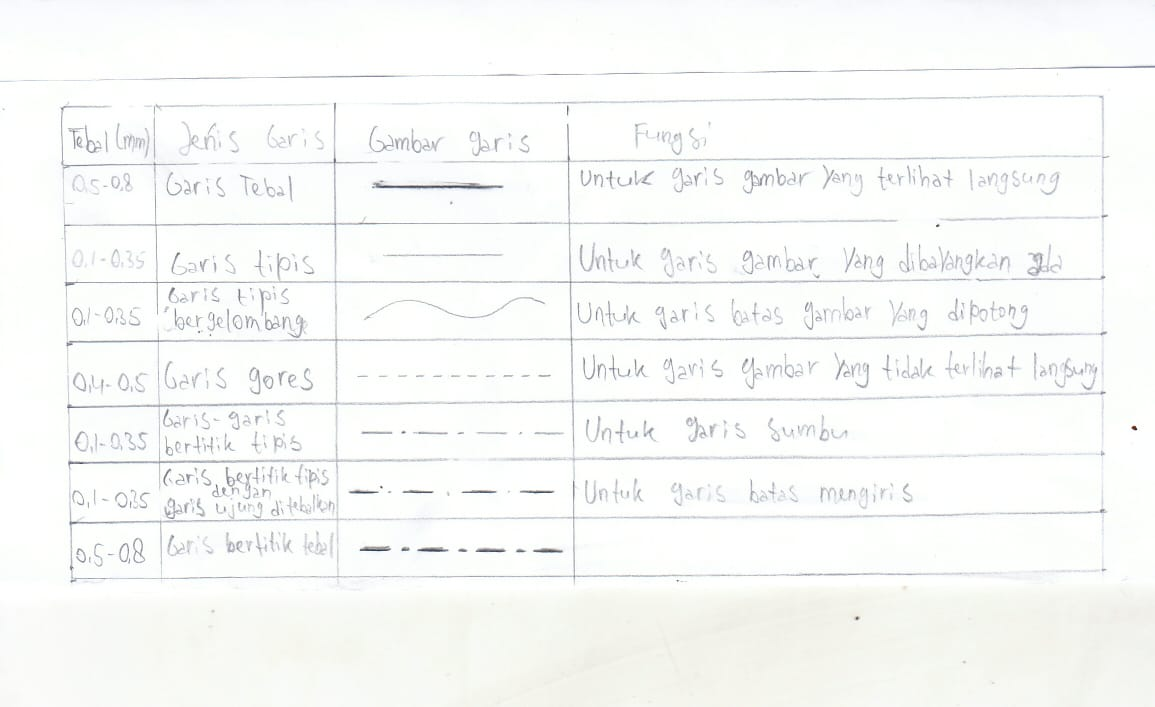
\includegraphics[width=0.8\textwidth]{../figures/tugasgaris.jpeg}
			\caption{Contoh gambar garis}
		\end{figure}
	\end{column}
	\begin{column}{.5\textwidth}
		\begin{figure}
			\centering
			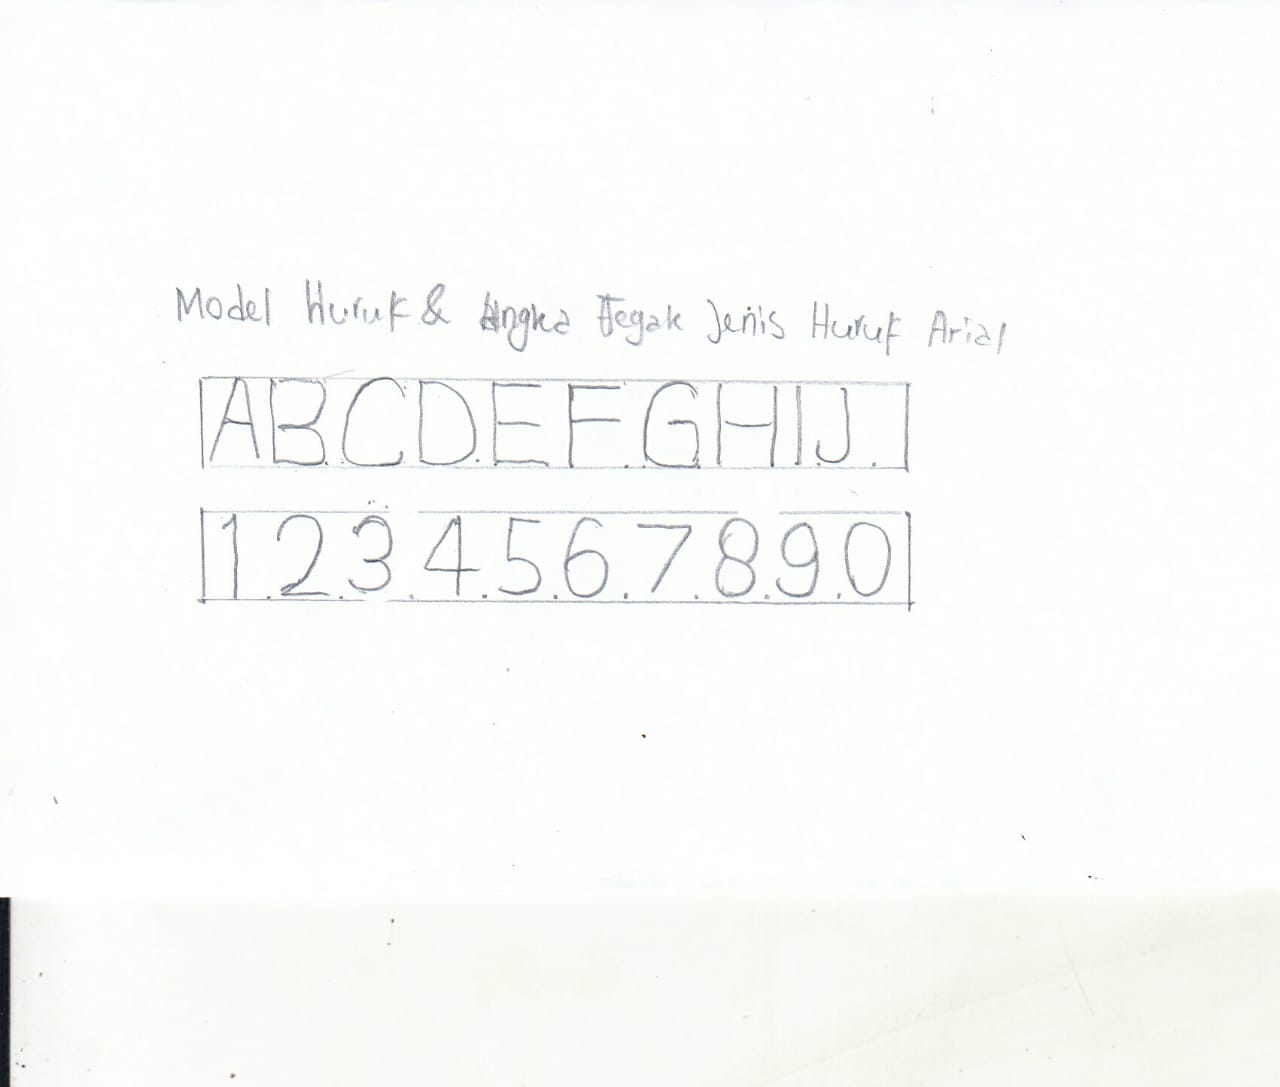
\includegraphics[width=0.8\textwidth]{../figures/tugashuruf.jpeg}
			\caption{Contoh Gambar huruf}
		\end{figure}
	\end{column}
\end{columns}

\subsection{Tugas rumah}%
\label{sub:Tugas rumah}

\textbf{Mata Kuliah} : Gambar Teknik\\
\textbf{Materi} : Pendahuluan Gambar Teknik

\subsubsection*{Petunjuk}
Jawablah pertanyaan berikut secara singkat, jelas, dan sistematis sesuai dengan materi yang telah dipelajari.

\subsubsection*{Soal Esai}

\begin{enumerate}
	\item Jelaskan mengapa gambar teknik disebut sebagai bahasa teknik dalam bidang permesinan.
	\item Sebutkan dan jelaskan dua fungsi utama gambar teknik dalam proses perencanaan dan pelaksanaan pekerjaan.
	\item Mengapa penggunaan standar (ukuran kertas, garis, dan skala) sangat penting dalam gambar teknik?
	\item Apa yang dimaksud dengan skala gambar, dan kapan skala pengecilan atau pembesaran digunakan?
	\item Menurut pendapat Anda, mengapa mahasiswa tetap perlu menggambar secara manual meskipun saat ini tersedia perangkat lunak CAD?
\end{enumerate}

\subsubsection*{Kunci Jawaban}

\begin{enumerate}

	\item Gambar teknik disebut bahasa teknik karena digunakan sebagai alat komunikasi visual untuk menyampaikan ide, bentuk, ukuran, dan cara pembuatan benda teknik secara jelas, baku, dan dapat dipahami oleh perencana maupun pelaksana.

	\item Dua fungsi utama gambar teknik adalah:
	      \begin{enumerate}
		      \item Menyampaikan informasi, yaitu sebagai media komunikasi antara perancang dan pelaksana pekerjaan.
		      \item Menuangkan gagasan, yaitu mengubah ide atau konsep perancang menjadi bentuk visual yang dapat diwujudkan.
	      \end{enumerate}

	\item Penggunaan standar dalam gambar teknik penting agar gambar seragam, jelas, dan tidak menimbulkan salah tafsir, sehingga mempermudah komunikasi, produksi, dan kerja sama.

	\item Skala gambar adalah perbandingan antara ukuran pada gambar dengan ukuran benda sebenarnya. Skala pengecilan digunakan jika benda terlalu besar, sedangkan skala pembesaran digunakan jika benda terlalu kecil agar detailnya terlihat jelas.

	\item Menggambar manual diperlukan untuk melatih ketelitian, pemahaman dasar gambar teknik, serta penguasaan aturan dan standar yang tetap menjadi dasar dalam penggambaran berbasis komputer.
\end{enumerate}






\bibliographystyle{apalike}
\bibliography{../filename.bib} % required for citecompletion, not work in mainfile
\end{document}

